\chapter{A Modern Tutorial on Geometric Deep Learning}
\label{ch:11-geometric-deep-learning}

\lecturemeta{Petar Veli\v{c}kovi\'{c}}{Google DeepMind and University of Cambridge}

The organising analogy is historical. In the nineteenth century geometry had fragmented into a
zoo of competing geometries, and Klein's Erlangen Program unified them by asking, for each one,
which group of transformations it leaves invariant. Veli\v{c}kovi\'{c} argues deep learning in the
2020s is in the same position, a zoo of architectures with no principle organising them, and
proposes the same remedy: specify the domain the data lives on and the group of symmetries acting
on it, then derive the admissible layers. The payoff claimed is not aesthetic. For several
architectures the derivation is tight enough to show that they \emph{must} have the form they do,
and the same recipe extends to domains where nobody has intuition, such as spheres and meshes.

\section*{Key ideas}

\paragraph{Invariance, equivariance, and why the second is the useful one.} A function is invariant
if the symmetry leaves its output unchanged, and equivariant if the output transforms
correspondingly. The definition given is that for $f : \dom \to \lab$, a group $\Grp$, and
representations $\rho_1$ and $\rho_2$ acting on the domain and codomain respectively, $f$ is
$\Grp$-equivariant when
\[
  f \circ \rho_1(g) = \rho_2(g) \circ f
  \qquad \text{for all } g \in \Grp,
\]
\noindent so applying the symmetry before $f$ is the same as applying it after. Invariance is the
special case $\rho_2 = \mathrm{id}$. The lecture's point is that
invariance is too strong to build with, because an invariant layer must collapse the whole input to
a single output and thereby throws structure away; so one stacks equivariant layers and takes an
invariant readout only at the end. Whether something is a symmetry is a property of the task, not
of the data: rotation is a symmetry for cats versus dogs and emphatically not for digit
recognition. Groups organise these symmetries, group actions turn them into operations on the
domain, and representations turn the actions into matrices, with $SO(2)$ rotations and $S_3$
permutations as the running examples.

\paragraph{The recipe.} Data lives on a domain $\Om$, an $N \times N$ grid, a set, a graph, and
the data itself is a signal $\Sig : \Om \to \mathcal{C}$. The key structural observation is that
an action on the domain induces an action on signals. Given that, the building blocks are linear
equivariant maps composed with local nonlinearities, and the derivation of each architecture is
just working out which linear maps are equivariant to the group in question. The lecture then works
this through for what it calls the four Gs: graphs, grids, groups and geometric graphs, with
manifolds and gauges as the finale, following the structure of the companion
book~\citep{bronstein2021gdl}.

\paragraph{Graphs give message passing, with no freedom left.} Permutation equivariance plus a
locality requirement forces the layer to be a function of a node and its neighbourhood, and the
result is the message-passing form
\[
  \vect{h}_u = \upd\Bigl(\xin_u, \;\agg_{v \in \nbr{u}} \msg(\xin_u, \xin_v)\Bigr),
\]
\noindent where $\msg$ is the message function, $\agg$ the aggregation and $\upd$ the update
(Figure~\ref{fig:geometric-deep-learning-1}). The only requirement on $\agg$ is permutation
invariance, so sum, max or mean all qualify, and message and update are the only parametric parts.
The lecture is explicit that this is derived rather than designed: locality is presented as
possibly the only way to satisfy equivariance without collapsing.

\begin{figure}[htbp]
\centering
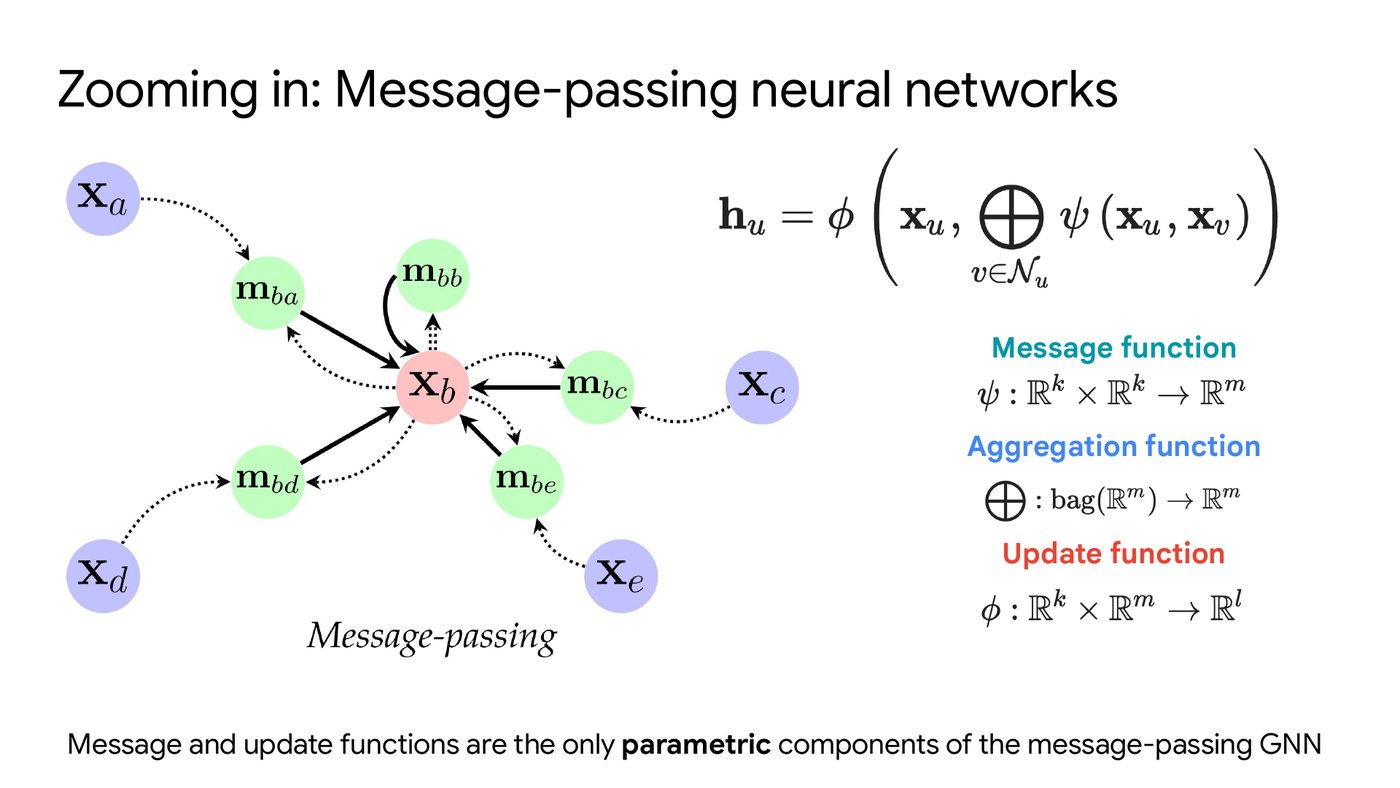
\includegraphics[width=0.86\textwidth]{figures/geometric-deep-learning-1.jpg}
\caption{The message-passing layer as derived in the Geometric Deep Learning tutorial. Node $b$
receives a message $\vect{m}_{bv}$ from each neighbour, the messages are combined by a
permutation-invariant aggregator, and the update produces $\vect{h}_u$. Only $\msg$ and $\upd$ carry
parameters; the aggregator's only job is to make the layer indifferent to neighbour ordering.}
\label{fig:geometric-deep-learning-1}
\end{figure}

\paragraph{Transformers are graph neural networks.} The most provocative section argues that
treating LLMs as sequence models is a category error. Nodes are tokens,
$V = \{1, \dots, N\}$, features are token embeddings, and the causal mask is precisely a
neighbourhood definition, $v \in \nbr{u} \iff v \le u$. Dot-product self-attention is then a
message function in two parts, with the softmax denominator handled by an aggregator that
accumulates both numerator and normaliser and an update that divides, so the whole block is an
MPNN on a complete or causally-masked graph~\citep{joshi2025}, with graph attention
networks~\citep{velickovic2018gat} credited on the slide as the attentional precursor. The practical
value is diagnostic: once a transformer is a GNN, its known pathologies become graph pathologies,
and the lecture names overmixing and oversquashing as exactly the phenomena the GNN literature has
studied. Both connect back to the DAG structure of causal attention in
Chapter~\ref{ch:09-spectral-analysis-dags}.

\begin{figure}[htbp]
\centering
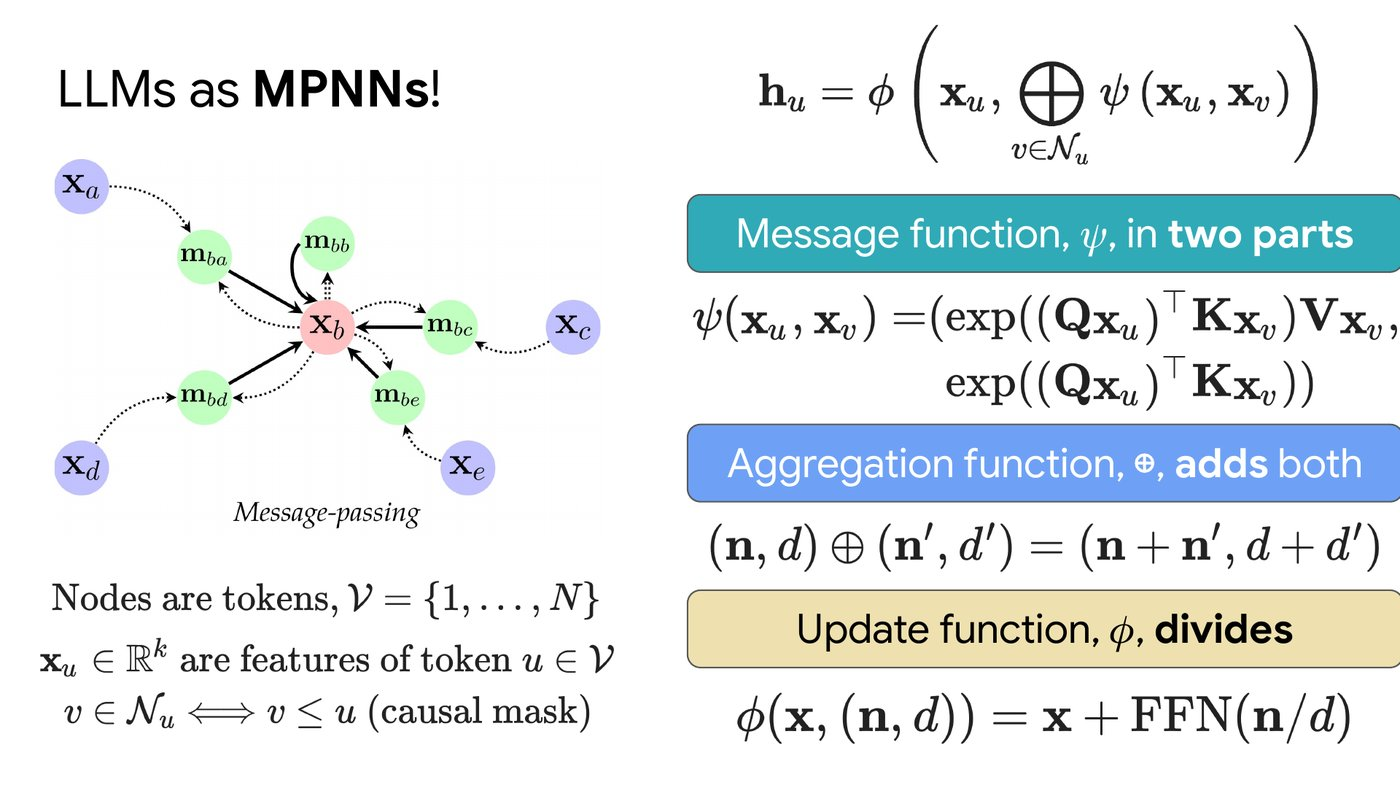
\includegraphics[width=0.86\textwidth]{figures/geometric-deep-learning-2.jpg}
\caption{A transformer block written as message passing, from the Geometric Deep Learning
tutorial. Nodes are tokens, $\nbr{u}$ is fixed by the causal mask $v \le u$, and the block decomposes
exactly into the three MPNN components. The message function carries two parts, the attention
numerator $\exp((\mat{Q}\xin_u)\T \mat{K}\xin_v)\mat{V}\xin_v$ and its denominator
$\exp((\mat{Q}\xin_u)\T \mat{K}\xin_v)$; the aggregator sums both componentwise,
$(\vect{n}, d) \oplus (\vect{n}', d') = (\vect{n} + \vect{n}', d + d')$; and the update performs the
softmax division and the residual feed-forward step,
$\upd(\xin, (\vect{n}, d)) = \xin + \mathrm{FFN}(\vect{n}/d)$.}
\label{fig:geometric-deep-learning-2}
\end{figure}

\paragraph{Grids give CNNs, and the derivation is the point.} A grid is a graph with more
regularity, so one may restrict attention to the special permutations that are translations.
Collecting the parameters of a translation-equivariant linear map into a matrix forces that matrix
to be circulant, and every circulant matrix is a convolution. The conclusion is stronger than
motivation: all linear translation-equivariant maps on a grid are convolutions, which is why CNNs
must have the form they do. The same style of argument recovers gating in recurrent networks from
invariance to time warping, which is a satisfying derivation of GRU and LSTM structure from a
symmetry rather than from engineering.

\paragraph{Groups, and building for domains that resist intuition.} Generalising convolution from
translations to an arbitrary group $\Grp$ gives group convolution~\citep{cohen2016group}, and the
subtlety flagged is that after the first layer the signals live on $\Grp$ rather than on the
original domain, which is what makes depth work. Spheres are the worked example: $\Om = \Sph^2$
with 3D rotation symmetry, layer one maps $\Sph^2 \to SO(3)$ and subsequent layers act on
$SO(3)$~\citep{cohen2018spherical}. The applied highlight is TacticAI
(Figure~\ref{fig:geometric-deep-learning-3}), where the relevant symmetry is the dihedral group
$D_2$, an approximate symmetry of a football pitch under reflection along each
axis~\citep{wang2024tacticai}. This is the result the personal notes record as predicting corner
outcomes several seconds ahead, and the reason it belongs in this lecture is that the pitch
symmetry is approximate, so the equivariance is a modelling choice rather than a fact.

\begin{figure}[htbp]
\centering
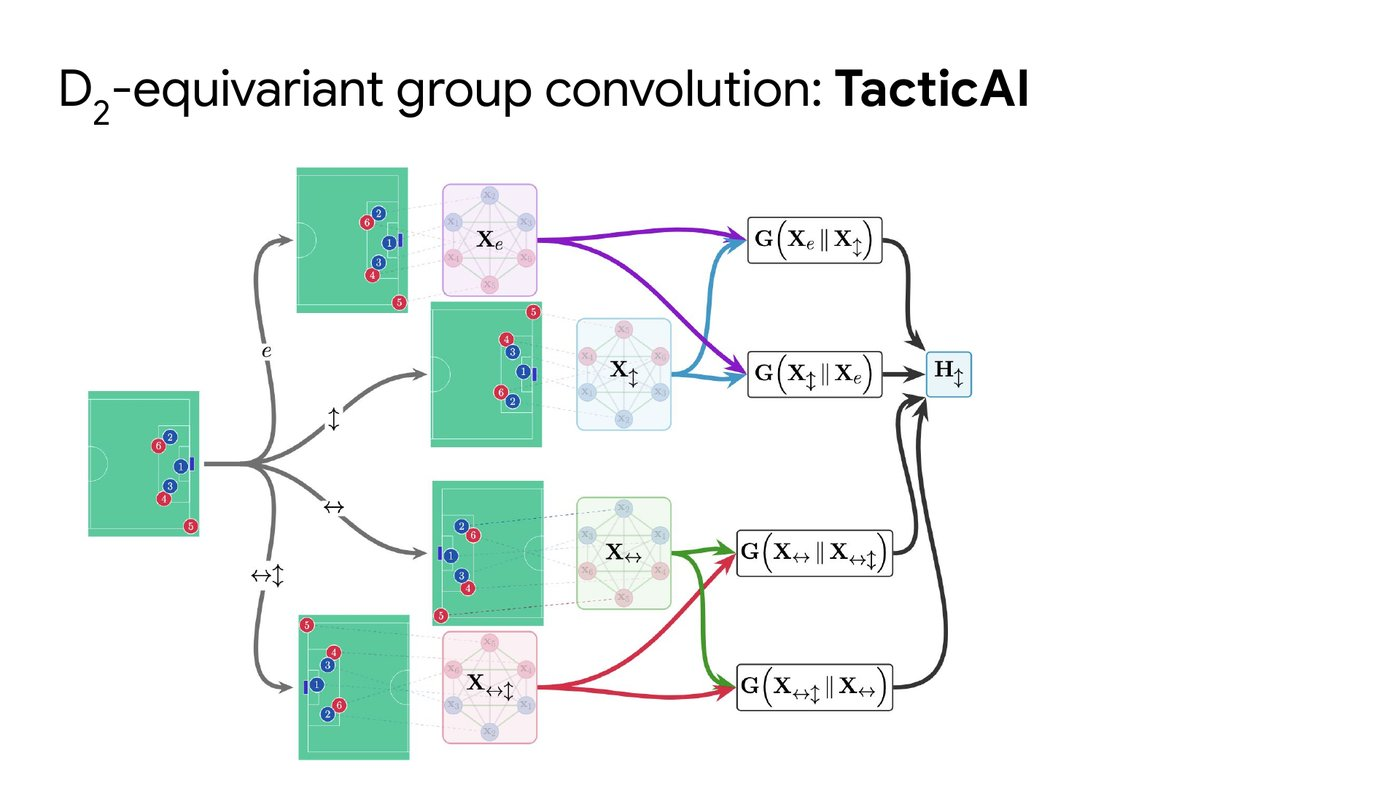
\includegraphics[width=0.88\textwidth]{figures/geometric-deep-learning-3.jpg}
\caption{Group convolution in the wild, from the Geometric Deep Learning tutorial. A corner-kick
configuration is transformed by each element of the dihedral group $D_2$, reflection along the
pitch's long axis, its short axis, and both, giving four views. Each is encoded, the encodings are
combined pairwise, and the result is pooled into a $D_2$-equivariant representation, so the model
cannot give a different answer merely because the play happened on the other side of the pitch.}
\label{fig:geometric-deep-learning-3}
\end{figure}

\paragraph{Geometric graphs, manifolds and gauges.} If the domain does not float in a vacuum but is
embedded in space, the relevant group is $E(3)$, roto-translation and reflection, combined with
permutation equivariance. The cheap route to guaranteed invariance is to message pass only on
invariant quantities such as pairwise distances; vector-valued features need genuinely equivariant
updates instead. Manifolds push this furthest. A 2D manifold is locally like $\R^2$, so one works
in the tangent space $T_u\Om$, moves along the surface with the exponential map $\exp_u X$, and
compares tangent vectors at different points by parallel transport $\Gamma_{u \to v}X$. Defining
convolution in the tangent space then runs into the central difficulty: the choice of gauge, the
local frame, is entirely arbitrary, and even on a sphere no consistent global choice exists.
Requiring gauge equivariance directly means conditioning across pairs of arbitrarily related
gauges, which the lecture calls very hard; parallel transporting features first simplifies it. The
resolution is deflationary and rather satisfying: what results is a GNN with extra precomputations
and angle-conditioned parameters, or as the slide puts it, just a graph with extra
structure. AlphaFold 2 carries the same ideas, maintaining a local frame per residue~\citep{jumper2021}
(Figure~\ref{fig:geometric-deep-learning-4}).

\begin{figure}[htbp]
\centering
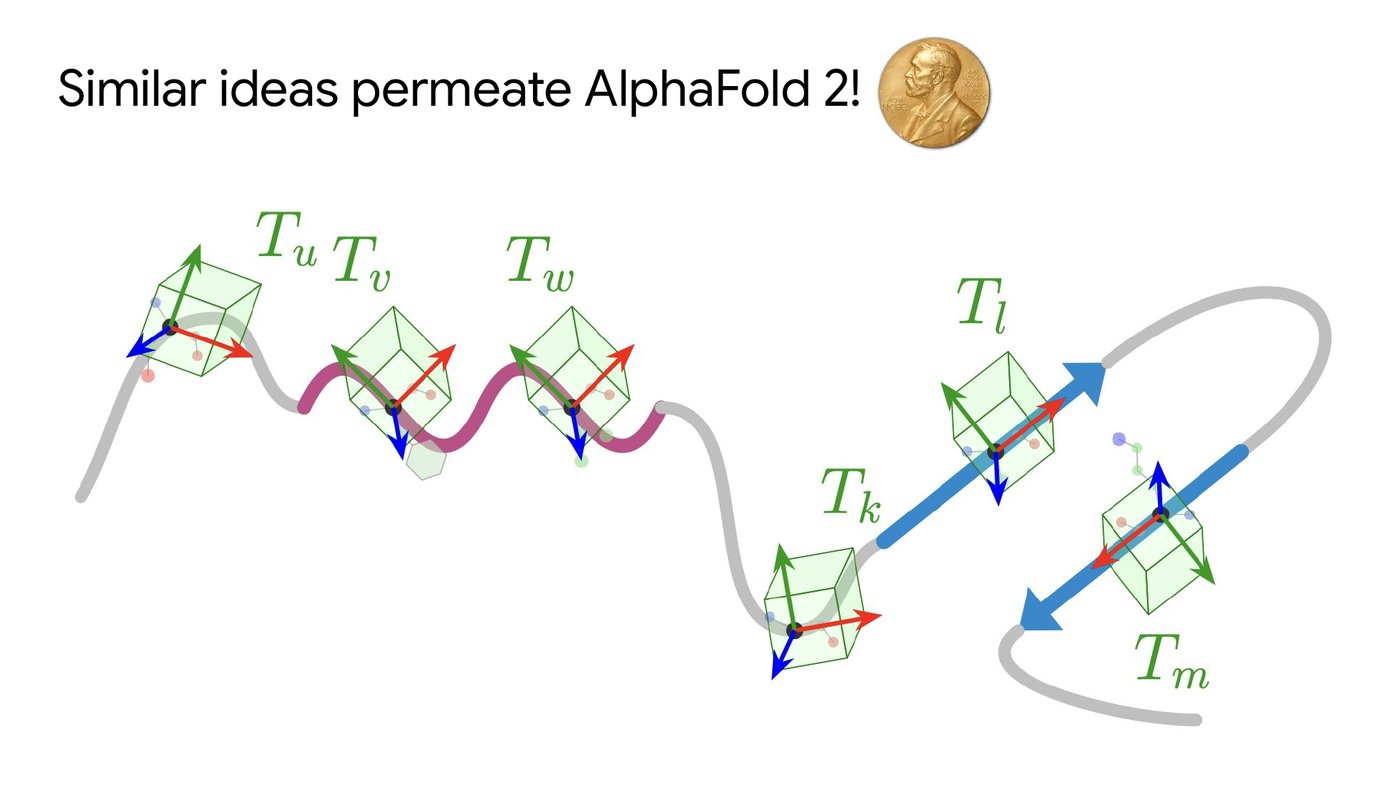
\includegraphics[width=0.82\textwidth]{figures/geometric-deep-learning-4.jpg}
\caption{Where the gauge machinery reappears, from the closing of the Geometric Deep Learning
tutorial. A protein backbone with a local coordinate frame $T_u, T_v, T_w, \dots$ attached to each
residue. Reasoning about relative geometry means transporting information between these frames,
which is the same problem as choosing gauges on a manifold. This is the slide the personal notes
record but whose image attachment is missing from disk; it is recovered here from the deck.}
\label{fig:geometric-deep-learning-4}
\end{figure}

\section*{Notation}

$\Om$ is the domain, $\Sig$ a signal on it, $\Grp$ a group with elements $g$, $\rho$ a
representation, $\nbr{u}$ the neighbourhood of node $u$, and $\msg$, $\agg$, $\upd$ the message,
aggregation and update functions. The slides write $\upd$ as $\phi$ and $\msg$ as $\psi$, and that
usage is kept here. Isola uses $\phi$ for a representation in
Chapter~\ref{ch:02-representational-geometry}, which is an unavoidable collision between two
speakers' conventions.

\section*{Why it matters}

This is the most explicitly unifying lecture of the week and it retroactively organises several
others. Cho's Set Transformer++ (Chapter~\ref{ch:05-statistics-estimation}) is a permutation
equivariant architecture derived exactly the way this lecture prescribes, without either speaker
citing the other. The Feynman-graph failure in
Chapter~\ref{ch:08-ml-for-mathematics}, where $\phi^4$ graphs are 4-regular and so message passing
is blind by 1-WL, is a case where this toolkit is the named fix. And the transformers-as-GNNs claim
is the bridge to Chapter~\ref{ch:09-spectral-analysis-dags}: if a causally-masked transformer is a
GNN on a DAG, then its adjacency spectrum collapses, and zero-padding is a candidate for
recovering it.

\begin{aside}
Two follow-ups from the personal notes belong here. The mathematical prerequisites are published
separately as a long companion on the group- and representation-theoretic background, recorded in
those notes as \url{https://arxiv.org/abs/2508.02723}, and the course home is
\url{https://geometricdeeplearning.com}, with the MIT Press book dated 2026 on the closing slide.
The direction of the dependency is worth noting: nothing in the four Gs requires that background in
order to be \emph{used}, but the derivations, which are the actual content of the lecture, do.
\end{aside}
